\subsection*{Задание 1.2}
	\paragraph{1)}
	При помощи команды \textit{pwd} можно определить абсолютный путь до текущего расположения. При помощи команды \textit{mkdir} мы создаем пустую папку \textit{/1}. C помощью команды \textit{cd} можно перемещаться по директориям.\\
	\\
	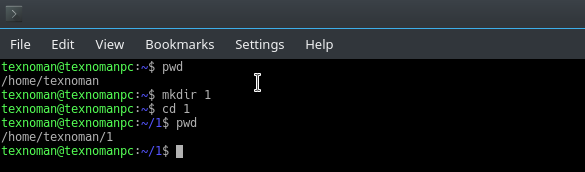
\includegraphics[width=\textwidth]{1.png}

	\paragraph{2)}
	Одновременно были созданны в \textit{/home/texnoman/1} папки \textit{Trufanova} и \textit{Antipov}. Подтвердили создание папки при помощи команды \textit{ls}( ключик \textit{-l} показывает размер, права на файл или папку, имя пользователя создавшего файл или папку).\\
	\\
	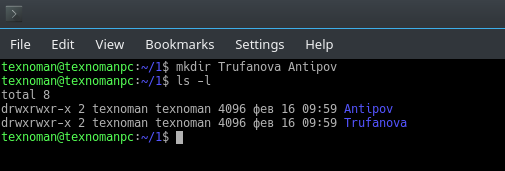
\includegraphics[width=\textwidth]{2.png}

	\paragraph{3)}
	Не переходя в директорию \textit{/home/texnoman/1/Antipov} была создана директория \textit{VladAnnaMakar}. Далее мы подтвердили создание папки с помощью команды \textit{ls}.\\
	\\
	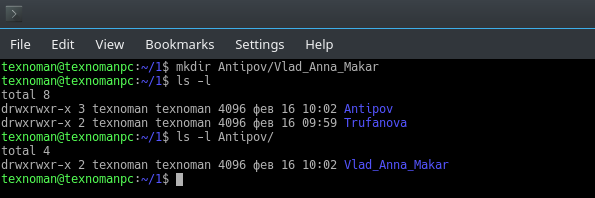
\includegraphics[width=\textwidth ]{3.png}

	\paragraph{4)}
	При помощи \textit{cd} мы перешли в папку \textit{/VladAnnaMakar}, используя относительный путь: \textit{Antipov/VladAnnaMakar} и одновременно были созданы два файла \textit{Vlad} и \textit{Anna} при помощи комманды \textit{touch}. Подтвердили создание файлов командой \textit{ls}. Отобразили текущий путь при помощи \textit{pwd}.\\
	\\
	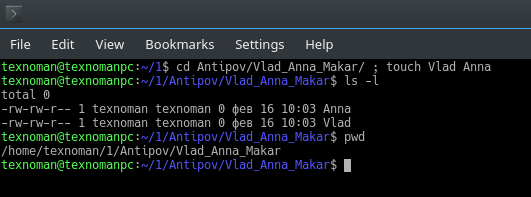
\includegraphics[width=\textwidth]{4.png}

	\paragraph{5)}
	При помощи команды \textit{touch}, указывая абсолютный путь, создаем файл с именем третьего участника (\textit{Makar}). При помощи \textit{ls} осуществляем проверку.\\
	\\
	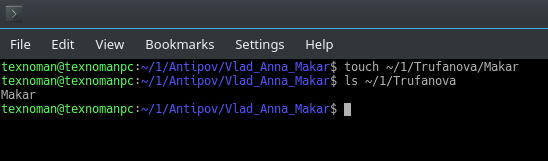
\includegraphics[width=\textwidth]{5.png}

	\paragraph{6)}
	При помощи команды \textit{cp} копируем директорию \textit{VladAnnaMakar} и всё её содержимое в папку \textit{./1}.
	Для того, чтобы скопировалось вместе со всем содержимым указываем флажок \textit{-r}.\\
	\\
	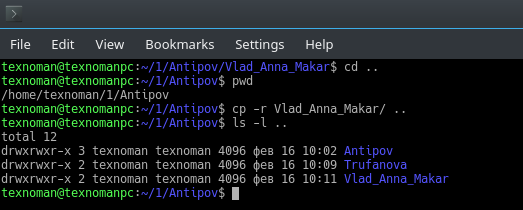
\includegraphics[width=\textwidth]{6.png}

	\paragraph{7)}
	Используя команду \textit{cp} копируем из директории \textit{VladAnnaMakar} файл \textit{Vlad} в папку \textit{Antipov}
	При помощи команды \textit{cd} перемещаемся в папку \textit{Antipov}(cd ..) и удаляем папку \textit{VladAnnaMakar/}. 
	При использовании флажка \textit{-r} рекурсивно удаляется все, что находится внутри директории. Проверяем с помощью 
	\textit{ls}.\\
	\\
	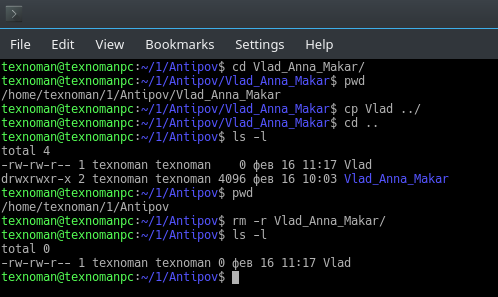
\includegraphics[width=\textwidth]{7.png}

	\paragraph{8)}
	Используя команду \textit{mv} переносим файл \textit{Makar} в папку \textit{./1}, переименовав его в файл \textit{Empty}.
	Подтверждаем нахождение файла с помощью \textit{ls}.\\
	\\
	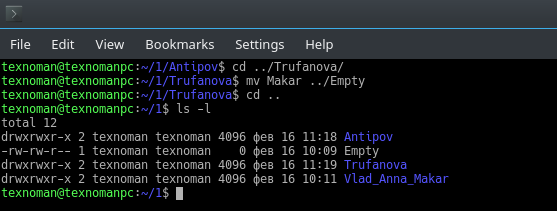
\includegraphics[width=\textwidth]{8.png}

	\paragraph{9)}
	При помощи команды \textit{mv} перемещаем все файлы, после чего используя команду \textit{rm}, удаляем имя не соответствующее названию папки (\textit{Vlad}).\\
	\\
	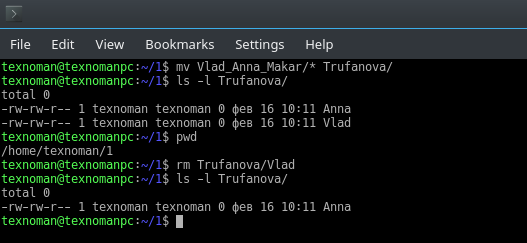
\includegraphics[width=\textwidth]{9.png}
	\\

	Удаляем пустую директорию при помощи команды \textit{rmdir}. Выводим рекурсивно содержимое папки \textit{/1} при помощи 
	\textit{ls -R}.\\
	\\
	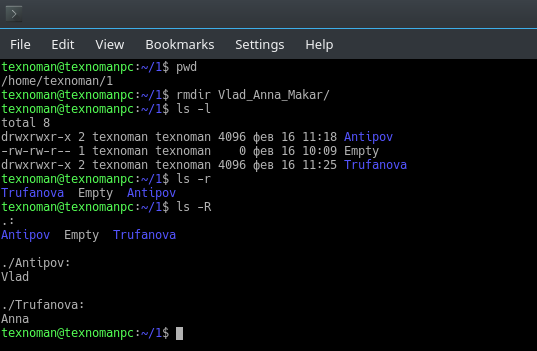
\includegraphics[width=\textwidth]{10.png}
	\\
	\\

	\paragraph{9)}
	Используя команду \textit{cd} и специальный знак - тильду перемещаемся в папку \textit{/1}. 
	Команда \textit{nano} открывает текстовый редактор nano,  в котором мы вводим необходимый текст. И сохраняем под названием \textit{finita}. Подтверждаем создание файла с помощью \textit{ls}\\
	\\
	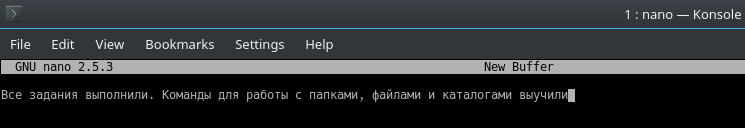
\includegraphics[width=\textwidth]{11.png}
	\\
	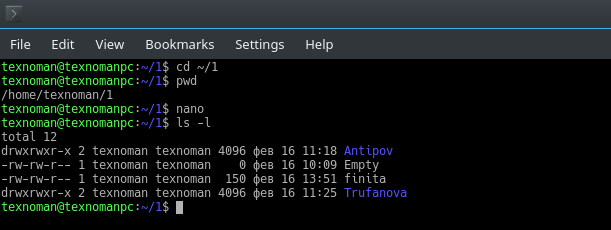
\includegraphics[width=\textwidth]{12.png}
	\\

	\paragraph{10)}
	Команда \textit{cat} позволяет прочитать содержимое файла(\textit{finita}).\\
	\\
	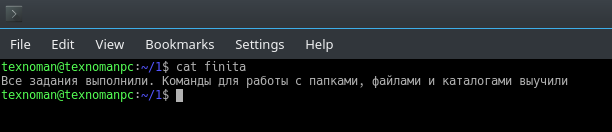
\includegraphics[width=\textwidth]{13.png}
	\\
	
	\paragraph{11)}
	Структура директории \textit{/home/texnoman/1} может быть получена с помощью \textit{ls -R}.\\
	\\
	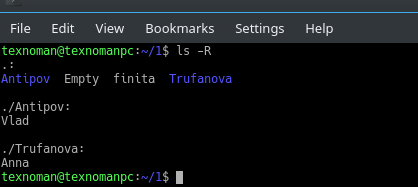
\includegraphics[width=\textwidth]{14.png}